\documentclass{article}
%\VignetteIndexEntry{Sushi}
\usepackage{Sweave}
\begin{document}
\begin{center}
\Large
{\tt Sushi} Package Vignette
\normalsize
\end{center}
The following figure illustrates the features of the plotManhattan function
\begin{Schunk}
\begin{Sinput}
> library('Sushi')
> Sushi_data = data(package = 'Sushi')
> data(list = Sushi_data$results[,3]) 
> # make color palette
> palette_fire_dark = colorRampPalette(c("black","blue","#5900E5","#E5001B","orange"))
> # set the margins
> par(mar=c(3,4,3,2))
> # set the genomic regions
> chrom1            = "chr11"
> chromstart1       = 500000
> chromend1         = 5050000
> chrom2            = "chr15"
> chromstart2       = 73000000
> chromend2         = 89500000
> # make the manhattan plot
> plotManhattan(bedfile=Sushi_GWAS.bed,pvalues=Sushi_GWAS.bed[,5],genome=Sushi_hg18_genome,col=palette_fire_dark(nrow(Sushi_hg18_genome)),cex=0.75)
> # add zoom 1
> zoomsregion(region=c(chromstart1,chromend1),chrom=chrom1,genome=Sushi_hg18_genome, zoomborder = "black", lty=2,lwd = 1,extend=c(0.07,0.2),wideextend=0.2,offsets=c(0,.535))
> # add zoom 2
> zoomsregion(region=c(chromstart2,chromend2),chrom=chrom2,genome=Sushi_hg18_genome, zoomborder = "black", lty=2,lwd = 1,extend=c(0.07,0.2),wideextend=0.2,offsets=c(.535,0))
> # add labels
> labelgenome(genome=Sushi_hg18_genome,side=1,scipen=20,n=4,scale="Mb",edgeblankfraction=0.20,line=.18,chromline=.5,scaleline=0.5)
> # add y-axis
> axis(side=2,las=2,tcl=.2)
> mtext("log10(P)",side=2,line=1.75,cex=.75,font=2)
> # Add plot label
> mtext("A)   GWAS",side=3, adj=-.025,line=1,font=2)
\end{Sinput}
\end{Schunk}
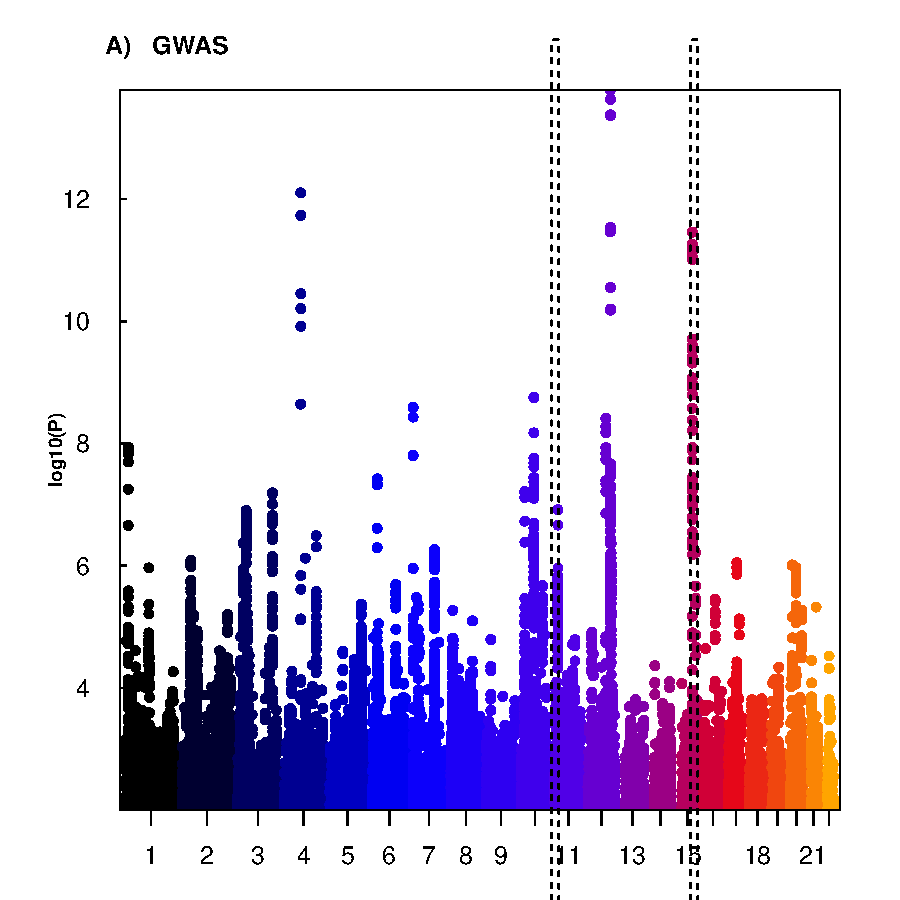
\includegraphics{Sushi-001}
\end{document}
